\section{Architecture matérielle du réseau}

%
%
\subsection{Architecture physique}

Après avoir vu l'architecture logique de notre réseau, nous pouvons maintenant établir l'architecture physique du réseau ainsi que le nombre d'équipements requis.

Tout d'abord, les deux bâtiments sont reliés à l'aide de deux fibres optiques de 100m (afin d'effectuer de la redondance en cas de coupure d'une de ces deux fibres) que l'on intègre dans le faux plafond du tunnel reliant les deux bâtiments.
Les fibres sont relié aux routeurs qui ce situant au N0. Elles sont connectées au routeur à l'aide de connecteur SFP+.

Le niveau -1 est le niveau où les scanners, radio s'effectuent ainsi que les opérations. Comme vue précédemment, il n'y a ni de WiFi, n'y d'accès à internet à ce niveau.
Les équipements médicaux étant branchés directement sur les ordinateurs a l'aide de câble console, on relie les ordinateurs ainsi que les téléphones au commutateur du niveau -1 situé dans un local prévu à cet effet.
De ce fait, les terminaux du niveau -1 font partie du VLAN Médical.

Au niveau 0, une salle est entièrement dédié aux équipements réseau. Cette salle contient une armoire. On y installe deux routeurs, deux lames serveur qui sont sur deux machines différentes, un NAS, un onduleur afin de palier aux pannes de courant ainsi que trois commutateurs.
Deux commutateurs de coeur de 24 ports où sont relié tous les équipements de l'infrastructure réseau et un commutateur 24 ports concernant le raccordement des terminaux du niveau 0.
Tous les équipements dans la salle sont doublés afin de garantir une haute disponibilité.

Il y a aussi  trois bornes WiFi, une fournissant internet pour les visiteurs et deux autres pour le personnel.
La borne WiFi fournissant internet pour les visiteurs fait partit du VLAN DonnéesVisiteur.
Les téléphones pour l'accueil et les bureaux administratif font partie du VLAN VoIPInterne.
Les ordinateurs et les bornes WiFi destinés aux personnels eux font partie du VLAN Données-Interne.

Le niveau 1 contient uniquement des terminaux faisant partit du VLAN Interne. Les terminaux téléphoniques font partie du VLAN VoIP-Interne, les ordinateurs et les deux bornes WiFi du VLAN Données-Interne. Tous les terminaux sont raccordés sur deux commutateurs de 24ports qui se situent dans le local de l'étage prévue à cet effet. Les équipements téléphoniques sont raccordés à un commutateur et les autres types de terminaux tels que les ordinateurs, bornes WiFi et prises RJ45 supplémentaires sur le deuxième commutateur.


Pour les niveaux de 2 à 4, on place une borne WiFi afin de fournir Internet aux patients. Cette borne fait partit du VLAN Données-Visiteur. Les téléphones pour les patients se situant dans chaque chambres font partie du VLAN VoIP-Visiteur.
Pour les médecins, infirmières, deux bornes WiFi sont mise en place et deux ordinateurs. Ces terminaux font partie du VLAN Données-Interne.
Deux téléphones sont aussi présent pour le personnel, ils font partie du VLAN VoIP-Interne.
Tous les terminaux sont raccordés à un commutateur. Du au grand nombre de terminaux à ces étages, deux commutateurs seront mis en place. Pour une question d'installation et de maintenance, tous les téléphones sont relié à un commutateur et les autres terminaux de type ordinateur et borne sont reliés au deuxième commutateur.

Les commutateurs se trouvant aux étages sont reliés directement sur les  deux commutateur de coeur qui se situe dans la salle du niveau 0.

Les téléphones et les bornes WiFi sont alimentés en PoE pour éviter d'installer des prises électriques à coté de ceux-ci.
Tous les raccordements sont fait à l'aide de câbles Ethernet SSTP catégorie 6 RJ45 sans halogène.

%
%
\subsection{Détails par étage}

    \begin{center}
        \begin{tabular}{|l|p{10cm}|r|}
          \hline
            Étages  &   Équipements    &   Prises RJ45 \\
          \hline
            N -1    &
            \begin{itemize}
                \item 6 Téléphones
                \item 8 Ordinateurs
                \item 1 commutateur 24ports
            \end{itemize}
            &   14 + 6 libres \\
          \hline
            N 0    &
            \begin{itemize}
                \item 3 Bornes WiFi
                \item 8 Téléphones
                \item 8 Ordinateurs
                \item 2 routeurs
                \item 2 Pare-feux logique
                \item 3 commutateur 24ports
                \item 1 NAS
            \end{itemize}
            &   16 + 4 libres \\
          \hline
            N 1    &
            \begin{itemize}
                \item 2 Bornes WiFi
                \item 9 Téléphones
                \item 9 Ordinateurs
                \item 2 commutateur 24ports
            \end{itemize}
            &   18 + 9 libres \\
          \hline
            N 2 à 4    &
            \begin{itemize}
                \item 3 Bornes WiFi
                \item 17 Téléphones
                \item 2 Ordinateurs
                \item 2 commutateur 24ports
            \end{itemize}
            &   19 + 2 libres \\
          \hline
        \end{tabular}
    \end{center}

%
    \cleardoublepage
%
%
\subsection{Schéma du réseau}

\begin{figure}[!ht]
    \center
    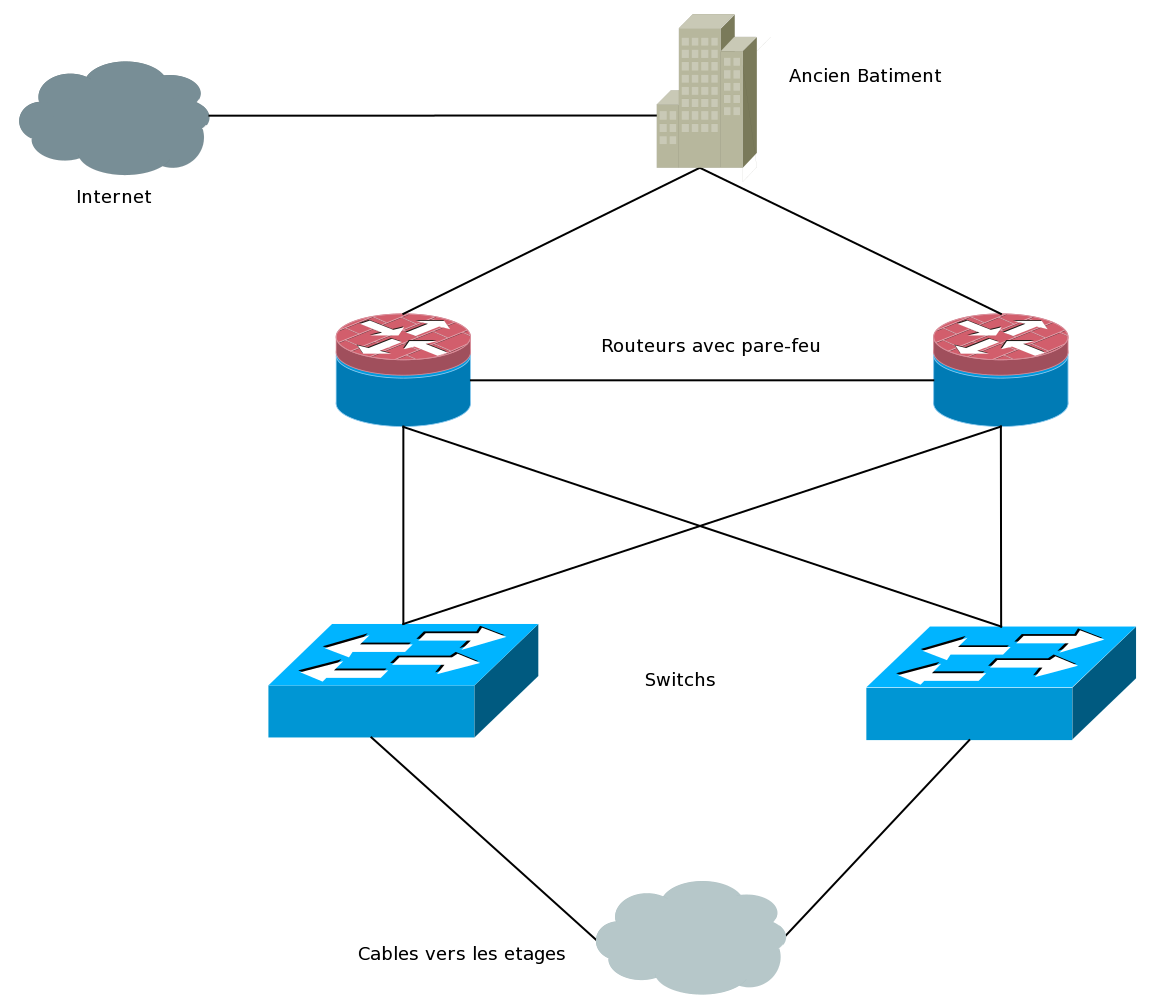
\includegraphics[width=1\textwidth]{./images/coeur-reseau.png}
    \caption{Schéma du coeur de réseau}
\end{figure}

\begin{figure}[!ht]
    \center
    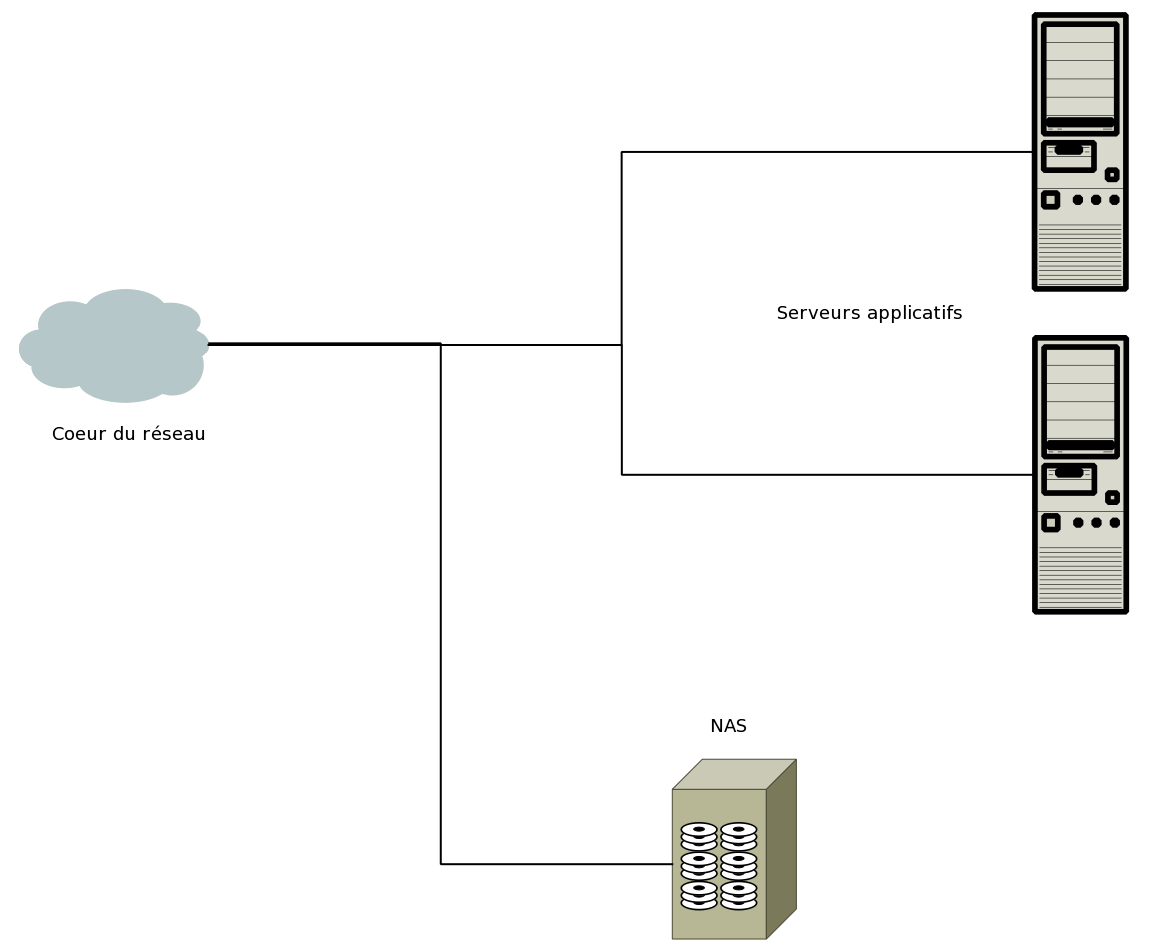
\includegraphics[width=1\textwidth]{./images/coeur-applicatif.png}
    \caption{Schéma du coeur applicatif}
\end{figure}

\begin{figure}[!ht]
    \center
    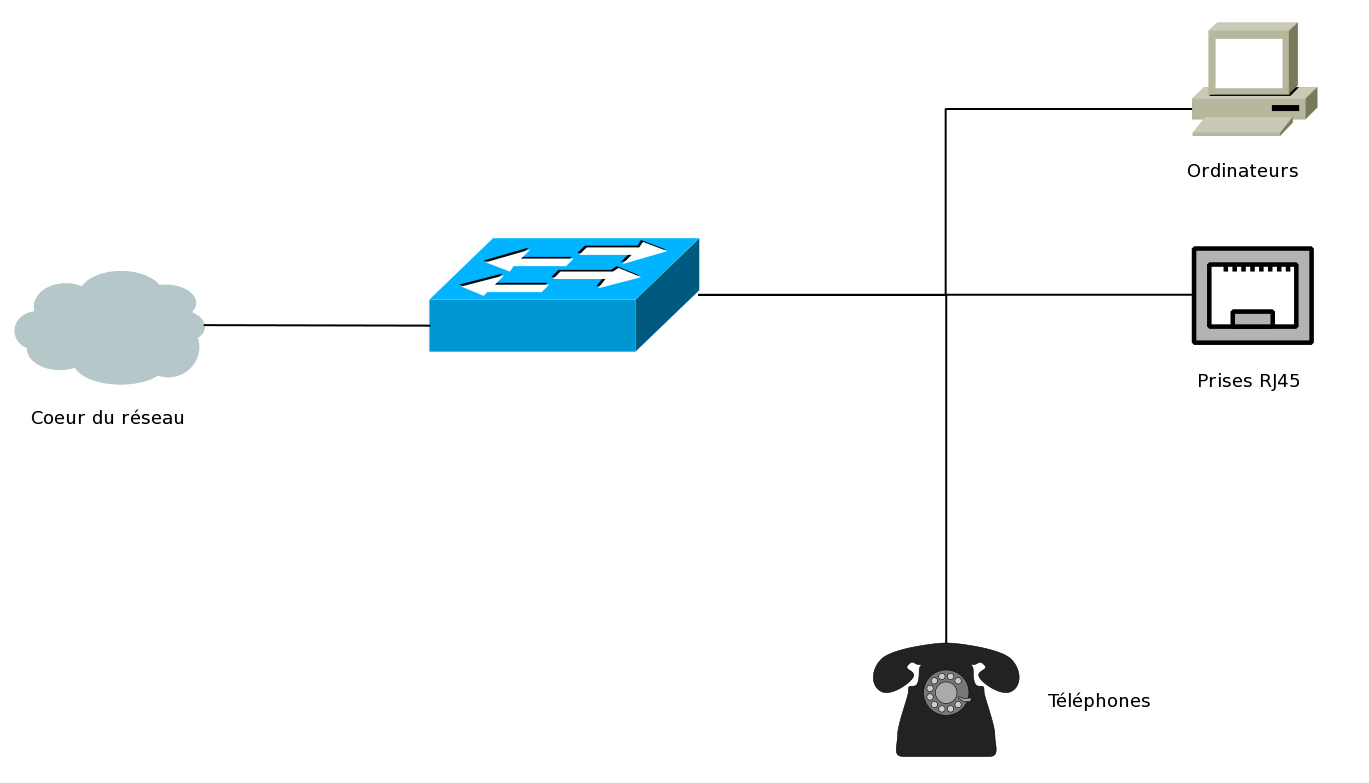
\includegraphics[width=1\textwidth]{./images/etage_n-1.png}
    \caption{Schéma du réseau au niveau -1}
\end{figure}

\begin{figure}[!ht]
    \center
    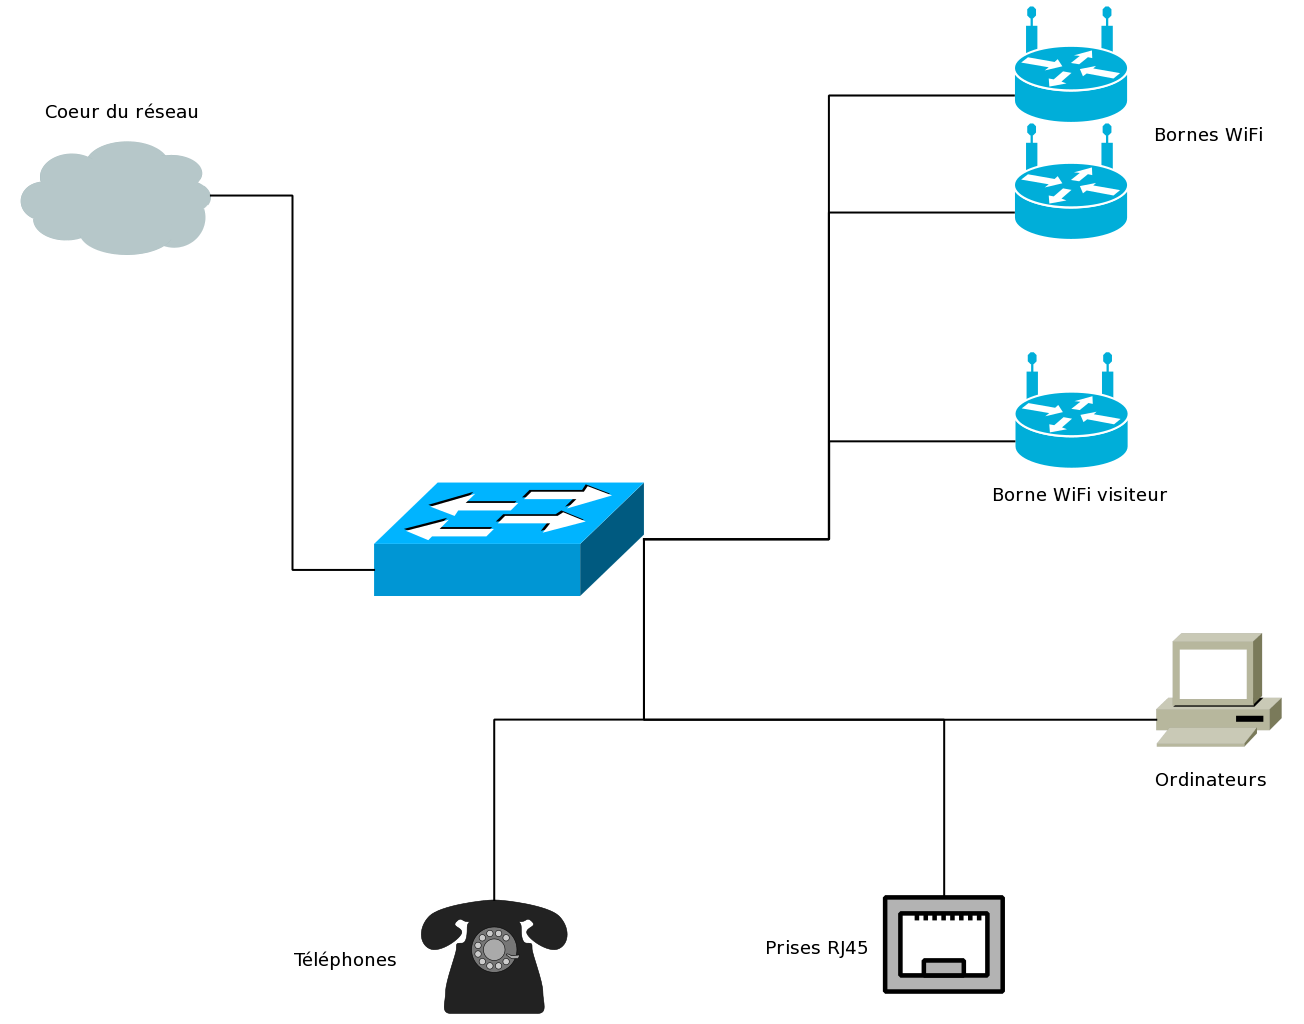
\includegraphics[width=1\textwidth]{./images/rez-de-chaussee.png}
    \caption{Schéma du réseau au rez-de-chaussée }
\end{figure}

\begin{figure}[!ht]
    \center
    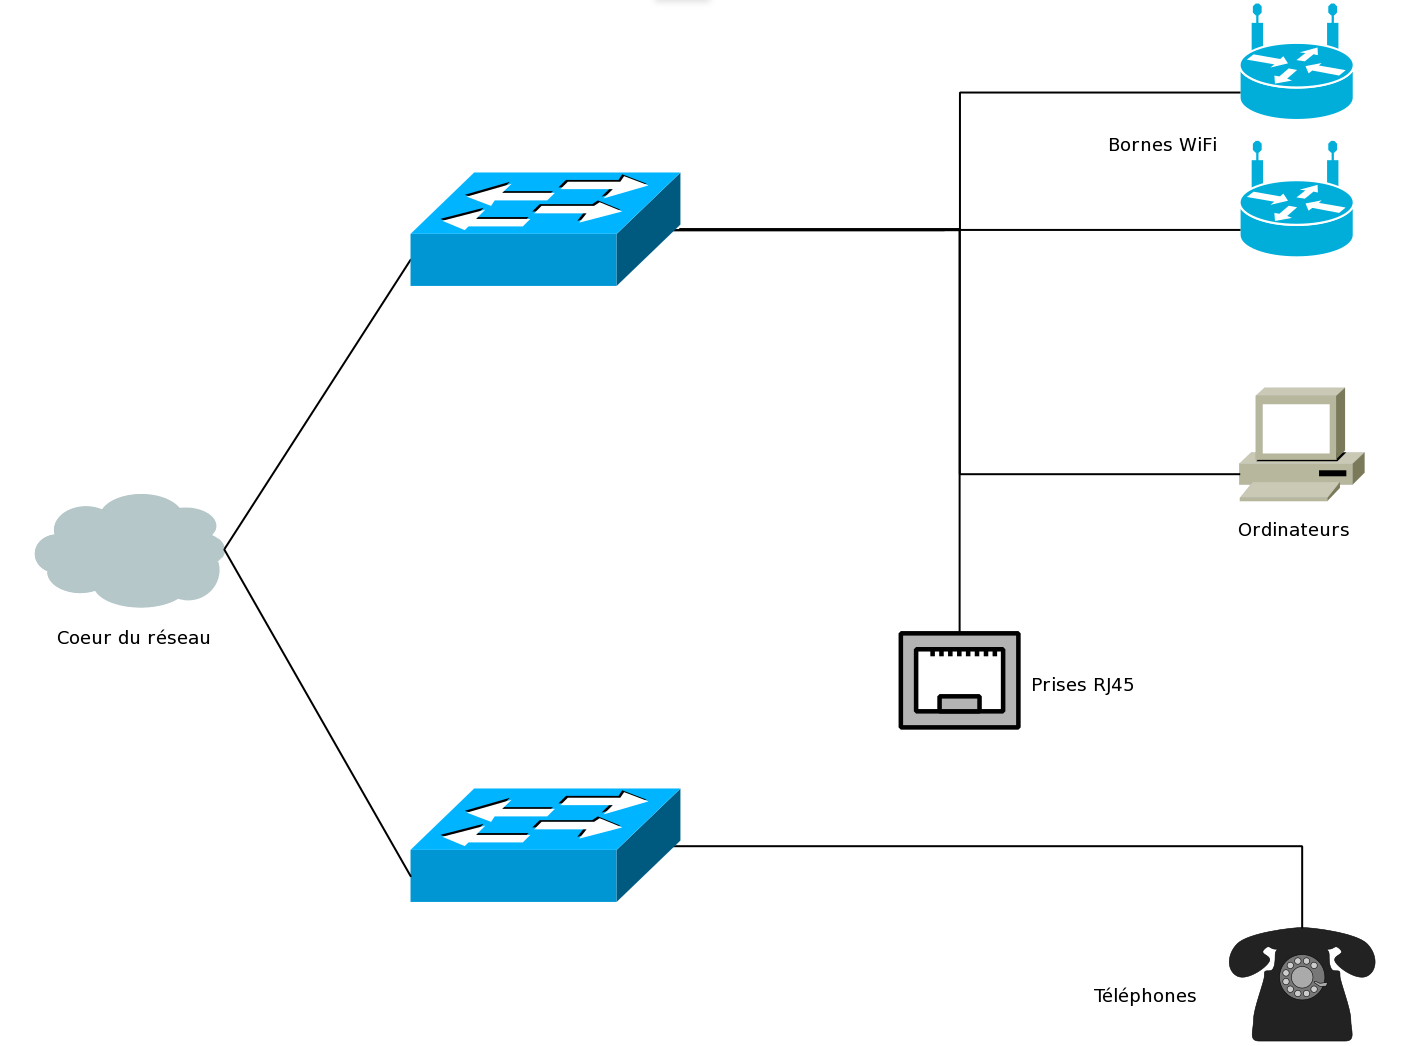
\includegraphics[width=1\textwidth]{./images/etage_n1.png}
    \caption{Schéma du réseau au premier étage}
\end{figure}

\begin{figure}[!ht]
    \center
    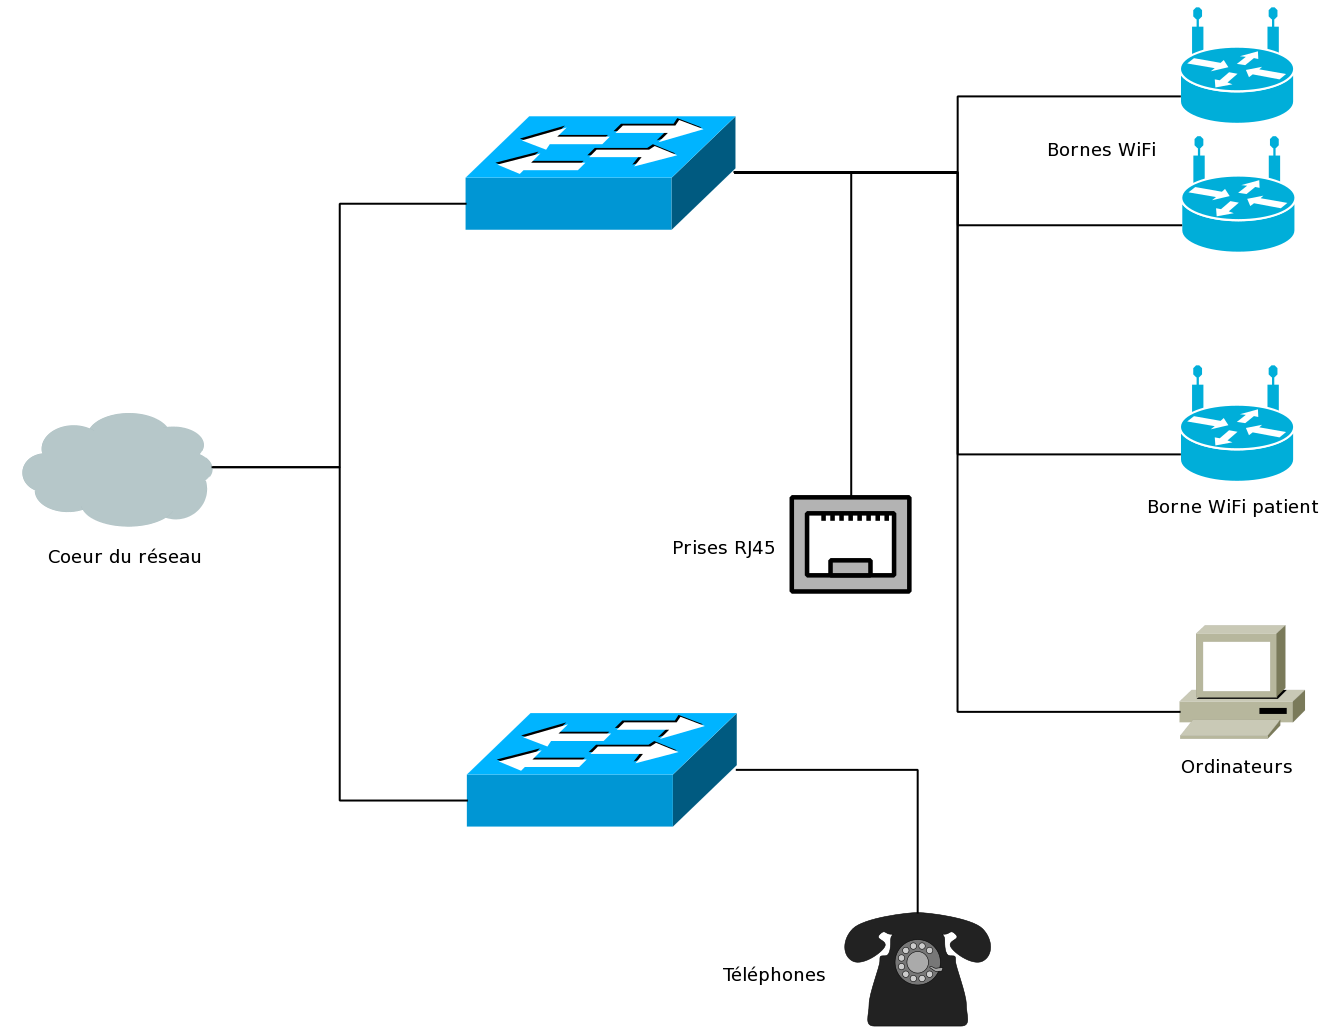
\includegraphics[width=1\textwidth]{./images/etage_n2-4.png}
    \caption{Schéma du réseau pour chacun des niveaux de 2 à 4}
\end{figure}

%
%

    \cleardoublepage

%
%
\subsection{Équipement du coeur du Réseau}

%
\subsubsection{Routeur}

Le besoin essentiel de nos routeurs est de pouvoir gérer chaque trames qui circulent dans le réseau.

Tout d'abord nos deux routeurs auront la même fonction, les mêmes services installés.
Pour cela l'équilibrage de charge de chacun d'eux permettra de limiter les pannes et faciliter la tolérance aux pannes. En effet dès lorsqu'un routeur est amené à être défaillant, l'autre routeur écoute celui-ci et sans retour, il prend l'initiative de prendre le relais. Les différents VLANs sont crées sur les routeurs.

Chaque routeur a la responsabilité d'administrer le coeur de réseau. Ils sont configurés pour assurer intégralement la sécurité et la gestion de routage du nouveau bâtiment.
Les ports 80 (navigateur Web consultation d'un site HTTP)  et 443 (sécurisé HTTPS utilisant la couche SSL) sont ouvert afin de gérer au mieux les requêtes. Un pare-feu UFW est lui aussi configuré pour simplifier la gestion des iptables. Pour finir un ensemble de protocoles destinés au routage au transport etc.. rendent le service d'un routeur totalement fonctionnel.

OSPF :
c'est un protocole de routage, or RIP a ses limites et OSPF répond à une dynamique de routage plus moderne. OSPF est à mettre en place dans chaque routeur pour faciliter le routage.
Les avantages de ce protocoles assurent ces bonnes caractéristiques :

Il n'y a pas de limite du nombre de sauts. Avec OSPF chaque routeur possède déjà une connaissance complète du réseau. Dès lors qu'il y a modification d'un lien ou ajout, une mise a jour des tables de routage se fait automatiquement.
Bien évidemment le protocole OSPF ne connaît que sa zone.
L'usage du VLSM améliore l'organisation du plan d'adressage. De même OSPF utilise une IP multicast pour envoyer à chaque routeur ses mises à jour d'état de lien.

Nous avons expliqué la fonctionnalité essentielle de la répartition de charges entre routeurs, mais aussi entre les serveurs lames que nous installerons. Nous pouvons dire également que OSPF assure un rendu efficace pour la répartition de charge. Contrairement à RIP, OSPF dispose d'une meilleure convergence des changements de routages grâce aux relations de voisinage qu'il affectionne.

%
\subsubsection{Serveurs d'applications}

Pare Feu :
Le choix de la configuration du pare-feu se fait en mode logiciel sur le routeur sélectionné.
En effet l'outil UFW qui est un mode de configuration permet de simplifier les iptables en ligne de commande.
Cet outil UFW propose donc une alternative à l'outil iptables en toute simplification.
Il est même possible de bénéficier d'une configuration automatique de UFW et gérer le pare-feu sans pour autant avoir manipulé le programme.
La configuration de UFW se fait sur les deux routeurs du coeur de réseau. Ce Pare-Feu assure la sécurité des accès Internet et filtre les entrées et sorties.

NAS :
c'est un serveur de stockage réseau appelé Network Attached Storage. Il s'agit d'un serveur de fichier autonome relié à un réseau. Contrairement à un SAN plus cher à l'achat traite au niveau de l'ensemble réseau à l'aide d'une capacité de stockage à grande quantité, il est  composé de commutateurs, un ensemble  de disques de stockage. Souvent le SAN est câblé par une fibre optique pour assurer la rapidité des échanges.
Dans un réseau restreint comme celui-ci, bénéficier d'un serveur de stockage NAS suffit amplement.

Voici les raisons :
Usage du stockage uniquement dans le réseau local de l'hôpital
Données sauvegardées sont à titre professionnelles (locales)
L'ensemble des données touche les informations de cet hôpital.

Le serveur NAS est à usage identique comme un serveur de fichiers. C'est pour cela qu'il fournit des services à travers un réseau dit IP.  Le NAS se configure via une interface Web  et via également un gestionnaire de fichiers Web.
Pour cela dans le réseau de stockage, il est possible d'avoir le choix de traiter des protocoles tels que :
le NFS (Network File System)
Le CIFS (Common Internet File System)
Le FTP (File Transfert Protocol)


%
%
\subsection{Équipement de distribution}

%
\subsubsection{Commutateurs}
Chacun de nos commutateur a pour rôle de bien diffuser les paquets. Ainsi chaque commutateur à cinq VLAN configurés pour bien différencier ceux-ci.

Explication de création de VLAN :
un commutateur de 24 ports a n ports tagger pour chaque VLAN.
Nous  nous contenterons de voir dot1q dans le cas présent. Toutefois il est bon de savoir que chacun a son propre fonctionnement. ISL pour sa part encapsule toute les trames, quelque soit le VLAN. dot1Q, lui ne fait qu'insérer un tag (un marqueur) dans l'entête de la trame ethernet … et uniquement sur les VLANs autres que le VLAN natif. (Le VLAN natif est celui utilisé par les protocoles comme CDP par exemple pour s'échanger les informations)

%
%
\subsection{Équipement d'accès}

%
\subsubsection{Bornes WiFi}
Nous proposons deux sortes de bornes Wi-Fi. Par conséquent deux usages bien différents sont à séparer pour bien sécuriser les zones d'accès de chaques personnes.

Pour cela, un accès est dédié en Wi-Fi pour les visiteurs appelés les patients. Cet accès propose une navigation internet sécurisée mais aussi limitée par un pare-feu UFW configuré à cet effet pour bloquer différentes navigations interdites (argent, téléchargement). La norme 802.11b est une norme la plus répandue est parfaite pour le besoin des patients et visiteurs. Elle propose un débit de 11 Mbps avec une portée de 300 mètres environs en lieu extérieur. Sa fréquence est de 2.4Ghz, avec 3 canaux radio disponibles.
Un deuxième réseau wifi est mis en place pour le personnel. Ainsi le personnel peut travailler dans un réseau sécurisé, performant et sans dysfonctionnement. La norme 802.11a permet d'obtenir un haut débit de 30 Mbps réels environs. Sa fréquence est de 5 Ghz, avec 8 canaux radio.

%
%
\subsection{QOS}

Mettre en place un équilibrage de charges sur chaque routeur à l'aide du principe du HeartBeat, chaque routeur mais aussi serveur lame écoutent son voisin. La répartition appellée en anglais “load Balançing” sert de rendre les services opérationnels en cas de défaillance d'un équipement. C'est pour cela que dans le cas d'un établissement hospitalier si un routeur ou un serveur n'est plus fonctionnel alors le second équipement pourra toujours répondre à la demande et fourni les ressources nécessaire telles que l'accès à la base de données, ou à internet.
